% !TeX root = main.tex

\documentclass[12pt,a4paper]{article}
\synctex=1  % pour utiliser gedit et evince

\usepackage[utf8]{inputenc}
\usepackage[T1]{fontenc}
\usepackage[french]{babel}
\usepackage{fancyhdr}
\usepackage{graphicx}
\usepackage{eurosym}
\usepackage{geometry}
\geometry{ hmargin=2.5cm, vmargin=2.5cm } 
\usepackage{color}
\usepackage{hyperref}
% \hypersetup{hidelinks}  %hidelinks devrait fonctionner plutot que les 4 lignes suivantes
\hypersetup{
    colorlinks=false,
    pdfborder={0 0 0},
}
\setlength{\parindent}{0cm}  % supprimer espace en début de paragraphe

% ---------------- MACRO ------------------
\def\RT#1#2{\href{https://www.rottentomatoes.com/m/#1/}{#2}}
\def\acteur#1#2{\href{https://www.rottentomatoes.com/celebrity/#1/}{#2}}
\def\TR#1#2{\href{http://www.telerama.fr/cinema/films/#1}{#2}} % pour les films
\def\TRtele#1#2{\href{http://television.telerama.fr/tele/films/#1}{#2}} % pour les téléfilms
\def\beau{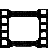
\includegraphics[width=0.025\textwidth]{icons/cadrage.png} }

% ------------- ACTEURS -------------------
\def\JackNicholson{\acteur{jack_nicholson}{Jack Nicholson}}
\def\DustinHoffman{\acteur{dustin_hoffman}{Dustin Hoffman}}
\def\RobertDeNiro{\acteur{robert_de_niro}{Robert De Niro}}
\def\KevinSpacey{\acteur{kevin_spacey}{Kevin Spacey}}
\def\ChristopherWalken{\acteur{christopher_walken}{Christopher Walken}}
\def\HarveyKeitel{\acteur{harvey_keitel}{Harvey Keitel}}
\def\JavierBardem{\acteur{javier_bardem}{Javier Bardem}}
\def\JohnMalkovich{\acteur{john_malkovich}{John Malkovich}}

% -------------- RÉALISATEURS --------------------
\def\RomanPolanski{\acteur{roman_polanski}{Roman Polanski}}
\def\TakeshiKitano{\acteur{takeshi_kitano}{Takeshi Kitano}}
\def\MartinScorsese{\acteur{martin_scorsese}{Martin Scorsese}}
\def\StanleyKubrick{\acteur{stanley_kubrick}{Stanley Kubrick}}
\def\JimJarmusch{\acteur{jim_jarmusch}{Jim Jarmusch}}
\def\DavidCronemberg{\acteur{david_cronemberg}{David Cronemberg}}
\def\FrancisFordCoppola{\acteur{francis_ford_coppola}{Francis Ford Coppola}}
\def\TerryGilliam{\acteur{terry_gilliam}{Terry Gilliam}}
\def\WoodyAllen{\acteur{woody_allen}{Woody Allen}}
\def\OrsonWelles{\acteur{orson_welles}{Orson Welles}}



% UTILISATION: \EXAMPLE{texte 1}{texte 2}
% -----------------------------------------------

\begin{document}

%\hyperlink{toc}{retour sommaire}  % lien table des matières, mais ça redimensionne la page

% LIEN URL:
%\href{         }{         } \\

% LIEN DANS LE DOC:
%\label{text:ancre}
%\hyperref[text:ancre]{First vers ancre}
% OU
%\hypertarget{terrygilliam}{terrygilliam}
%\hyperlink{terrygilliam}{(Terry Gilliam)}
 

\tableofcontents

\newpage
\section*{Nota Bene}
Ecrit en \LaTeX. Dernière mise à jour: 9/11/2013  \\
Cette liste regroupe tous les films qui m'ont particulièrement plu, pour une raison ou pour une autre. \\
Pour chaque catégorie, les films sont globalement classés par ordre de préférence (les meilleurs en premier) \\
\textcolor{blue}{Bleu = film admis comme culte, à avoir vu au moins une fois} \\
\textcolor{red}{Rouge = pas forcément culte mais le mériterait d'après moi, original, à voir}\\
\beau : film à l'esthétique très travaillé (2x l’icône =  excellent cadrage en plus) \\
Pour la plupart des films, cliquez sur le titre pour aller sur leur page \href{https://www.rottentomatoes.com/}{RottenTomatoes} ou \href{http://www.telerama.fr/}{Télérama} (pour certains les deux, ça dépend où vous cliquez sur le titre). \\
De même pour les acteurs. Vous pouvez ensuite voir quels sont leurs meilleurs films en cliquant sur "Rating". Exemple avec \RobertDeNiro: \\

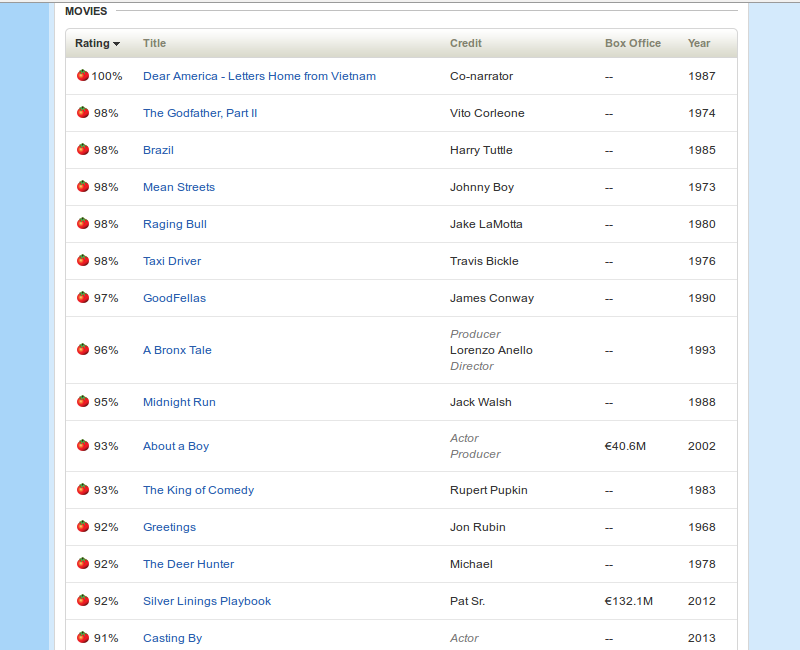
\includegraphics[width=0.9\textwidth]{divers/exemple1.png} 

\newpage
\section{Films étrangers}

\subsection{Drames}
\RT{graduate}{\textcolor{blue}{Le}} 
\TR{le-laureat,28082.php}{\textcolor{blue}{Lauréat}} 
(1967, Mike Nichols) \beau \beau \\
\RT{shame_2011/}{Shame} (2011, Steve McQueen, avec Michael Fassbender) \beau \beau \\
\TR{21-grammes,151627.php}{21 Grammes}
 (Innarritu, avec Sean Penn, Naomi Watts, Benicio del Toro) \\
Babel (Inarritu) \\
\TR{mar-adentro-mourir-pour-vivre,205498.php}{Mar Adentro} (Alejandro Amenabar, avec \JavierBardem) \\
\RT{tetro}{Tetro} (FF Coppola) \beau \\
\RT{1005199-dangerous_liaisons}{Les Liaisons Dangereuses} (avec \JohnMalkovich) \beau \\
\RT{1017834-romeo_and_juliet}{Roméo et Juliette} (1968, Zeffirelli) \\
\RT{10008466-deep_end}{\textcolor{red}{Deep End}} (1970) \beau \beau \\
\TR{two-lovers,358856.php}{Two}
\RT{two_lovers}{Lovers} (avec Joaquin Phoenix) \beau \\
Bright Star \beau  \\
\RT{taxi_driver}{\textcolor{blue}{Taxi Driver}} 
 (et autres de \MartinScorsese (surtout Les Affranchis)) \\
The Constant Gardener (avec Ralph Fiennes) \\
\RT{aguirre_the_wrath_of_god}{\textcolor{red}{Aguirre, la Colère de Dieu}}
 (1972, Werner Herzog, avec Klaus Kinski) \\
\RT{mulholland_dr}{Mulholland Drive} (David Lynch)\\
\RT{kramer_vs_kramer}{Kramer contre}
\TR{kramer-contre-kramer,6814.php}{Kramer} 
(avec \DustinHoffman, Meryl Streep) \\
Paranoid Park \\
\RT{lawrence_of_arabia}{Laurence d'Arabie} (1962, David Lean, avec Peter O'Toole) \\
\RT{dogville}{Dogville}  (2003, Lars Von Trier, avec Nicole Kidman) --> mise en scène originale\\
This is England \\
\RT{queen}{The Queen} (Stephen Frears) \beau \\
\RT{last_king_of_scotland}{Le Dernier Roi d'Ecosse} (2006, avec Forest Whitaker)\\
\RT{sex_lies_and_videotape}{Sex, Lies and Videotape} (1989, Steven Soderbergh)\\
Minuit dans le Jardin du Bien et du Mal (Clint Eastwood) --> esthétique bof mais scénario+ \\ \\

Drame bien genre on s'en souvient après, mais qui traîne un peu en longueur:\\
\RT{disgrace/}{Disgrace} (2008, avec \JohnMalkovich \\ 
\TR{la-porte-du-paradis,481506.php}{La Porte du Paradis} (1980) (Michael Cimino) \\

\subsection{Comédies}
\begin{tabular}{c c}
\begin{minipage}{12cm}
Midnight in Paris (et autres de \WoodyAllen) \beau \\
The Darjeeling Limited \\
\RT{lost_in_translation}{Lost in Translation} (2003, Sofia Coppola) \beau \\
\RT{juno}{Juno} \\
\RT{big_lebowski}{\textcolor{blue}{The Big Lebowski}}   (et autres des frères Coen) \\
\RT{clerks}{\textcolor{blue}{Clerks, les employés modèles}} (1994)\\
\RT{kiss_kiss_bang_bang}{Kiss Kiss Bang Bang} \\
Thank You for Smoking (avec Aaron Eckhart) \\
\TRtele{kaboom,19234405.php}{Kaboom} (2010, Greg Araki) \\
\RT{zombieland}{Zombieland} (2009) \\
\RT{tootsie}{Tootsie} (1982) --> pour \DustinHoffman \href{http://www.rue89.com/rue89-culture/zapnet/2013/07/10/dustin-hoffman-crois-suis-femme-interessante-244106}{(et voir ici)}\\
Le Tigre et la Neige (Roberto Benigni) \\
\end{minipage}
\begin{tabular}{c}
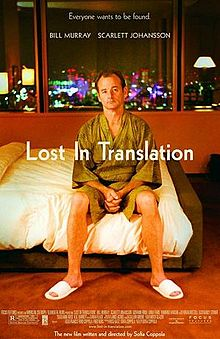
\includegraphics[width=0.25\textwidth]{affiches/lost.jpg}
\end{tabular} 
\end{tabular}


\subsection{Comédies dramatiques}
\RT{volver}{Volver} (2006) (et autres de Pedro Almodovar) \beau \\
\RT{wings_of_desire}{Les Ailes du Désir} (1987, Wim Wenders) \\
\RT{thelma_and_louise}{Thelma et Louise} (1991, Ridley Scott) \\

\subsection{Comédies romantiques}
\RT{ted_2012}{Ted} (2012) \\


\subsection{Parodique/second degré}
\textcolor{red}{Sugarland Express} (1974, Steven Spielberg) \\
\RT{machete}{\textcolor{red}{Machete}}  (2010, Robert Rodriguez) \\
\TR{perdita-durango,45065.php}{Perdita Durango}  (1997, avec \JavierBardem) \\
From Dusk till Dawn (1996, Robert Rodriguez, avec \HarveyKeitel)\\

\subsection{Aventure/road-movie}
\RT{crouching_tiger_hidden_dragon}{Tigre et Dragon} (2000, Ang Lee) \beau \\
\RT{into_the_wild}{Into The Wild} (2007, Sean Penn) \\

\subsection{Policier/Thriller}
\RT{ghost_dog_the_way_of_the_samurai}{Ghost}
\href{http://www.telerama.fr/cinema/films/ghost-dog-la-voie-du-samourai,46863.php}{Dog}
(1999, avec Forest Whitaker) (et autres de \JimJarmusch) \\
\RT{the_name_of_the_rose_1986}{Le Nom de la Rose}
 (JJ Annaud, avec Sean Connery, Michael Lonsdale...) \\
\RT{three_days_of_the_condor}{Les Trois Jours du Condor}
 (Sydney Pollack, avec Robert Redford) \\
\RT{marathon_man}{Marathon Man}   (avec \DustinHoffman, Michael Caine)\\
The Girl with the Dragon Tattoo (David Fincher)\\
Zodiac (David Fincher)\\
\RT{la_confidential}{L.A. Confidential} (avec Kevin Spacey)\\
\RT{mystic_river}{Mystic River} (2003, Clint Eastwood, avec Sean Penn)\\
Collateral (Michael Mann)\\
\RT{thomas_crown_affair}{L'Affaire Thomas Crown} (l'original de 1968 , avec Steve McQueen, Faye Dunaway) \beau \\
\RT{1114154-insomnia}{Insomnia} (Christopher Nolan, avec Al Pacino)\\
\TR{cosmopolis,434015.php}{Cosmopolis} (et autres de \DavidCronemberg)\\
The Pledge (Sean Penn, avec \JackNicholson)\\
\RT{king_of_new_york}{King of New York} (1990) (le meilleur rôle de \ChristopherWalken) \beau \\
Aniki mon Frère (et autres de \TakeshiKitano)\\
\RT{1023854-witness}{Witness} (Peter Weier, avec Harrison Ford)\\
\RT{cop_land}{Copland} (1997, avec Ray Liotta, \HarveyKeitel)\\
\RT{sin_city}{Sin City} (2005) \\
\RT{oldboy}{OldBoy} (2004) \\
La Corde (Hitchcock) \\

\subsection{Bon scénario/Twist}
The Truman Show \\
Eternal Sunshine (et autres de Michel Gondry) \beau \\
Memento (Christopher Nolan)\\
\RT{existenz}{eXistenZ}
 (\DavidCronemberg, avec Jude Law, Jennifer Jason Leigh, Willem Dafoe)\\
Inception (Christopher Nolan)\\
Shutter Island (\MartinScorsese)\\
\TR{le-limier-sleuth,332335.php}{Le Limier}
 (le remake, à défaut)(Kenneth Branagh, avec Jude Law, Michael Caine)\\
Dans la peau de John Malkovich (avec \JohnMalkovich)\\
Usual Suspects (avec Kevin Spacey)\\
\RT{1006345-duel}{\textcolor{blue}{Duel}}  (Spielberg)\\
Un Jour sans Fin (avec Bill Murray)\\
\RT{man_from_earth}{The Man from Earth}  (tout repose sur le scénario, très original)\\


\subsection{Science-Fiction}
\begin{tabular}{c c}
\begin{minipage}{12cm}
\RT{1003033-brazil}{\textcolor{blue}{Brazil}} (\TerryGilliam) \\
\RT{blade_runner}{\textcolor{blue}{Blade Runner}} (Ridley Scott, avec Harrison Ford) \beau \\
\RT{gattaca}{\textcolor{blue}{Bienvenue à Gattaca}}  (avec Ethan Hawke, Jude Law) \\
\RT{1016397-planet_of_the_apes}{La Planète des Singes} (l'original, avec Charlton Heston) \\
\RT{district_9}{District 9} (2009) \\
\RT{soylent_green}{\textcolor{red}{Soleil Vert}} (1973, avec Charlton Heston) \\
\RT{10009075-moon}{Moon} (2009) \beau \\
\RT{alien}{\textcolor{blue}{Alien}} (1979, Ridley Scott) \\
\TR{alien-la-r-surrection,27380.php}{Alien IV}
(JP Jeunet) \\
\RT{1000085-2001_a_space_odyssey}{\textcolor{blue}{2001 A Space Odyssey}}  (\StanleyKubrick) \\
\RT{thx_1138}{THX 1138}  (1971, Georges Lucas) \\
\RT{island}{The Island} (2005) (voir juste la première heure, après c'est nul) \\
\end{minipage}
\begin{tabular}{c}
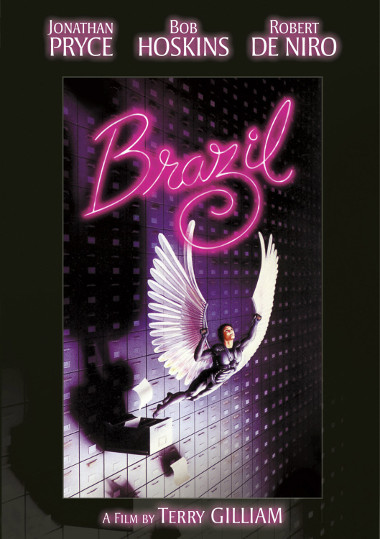
\includegraphics[width=0.25\textwidth]{affiches/brazil.jpg}
\end{tabular} 
\end{tabular}

\newpage
\begin{tabular}{c c c}
\begin{minipage}{5cm}
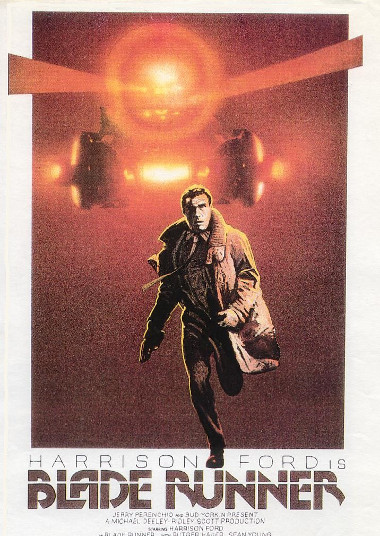
\includegraphics[width=0.9\textwidth]{affiches/bladerunner.jpg}  
\end{minipage} &
\begin{minipage}{5cm}
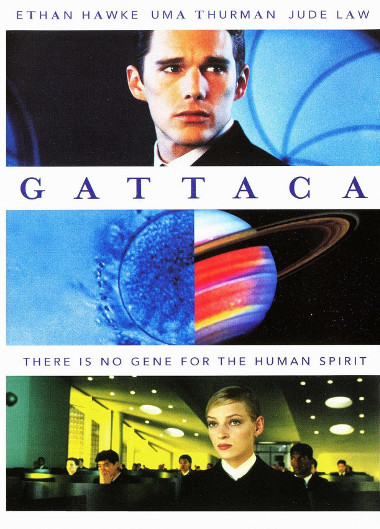
\includegraphics[width=0.9\textwidth]{affiches/gattaca.jpg}
\end{minipage} &
\begin{minipage}{5cm}
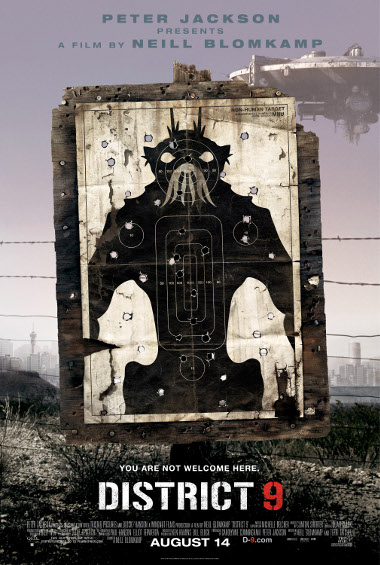
\includegraphics[width=0.9\textwidth]{affiches/D9.jpg} 
\end{minipage} \\ \\ \\
\end{tabular}

\subsection{Fantastique}
\RT{company_of_wolves}{La Compagnie des Loups} (1984)\\
\RT{arizona_dream}{\textcolor{blue}{Arizona Dream}}
 (1993, Kusturica, avec Johnny Depp) (très bonne musique)\\
Edward aux mains d'argent\\
\href{http://www.imdb.com/title/tt0460791}{The Fall} (2006)

\subsubsection*{Vampires}
\RT{the_fearless_vampire_killers}{Le Bal des Vampires} (1967, \RomanPolanski) (parodique) \beau \\
\RT{nosferatu}{Nosferatu} (1922, Murnau)\\
\RT{interview_with_the_vampire}{Entretien avec un Vampire} (1994)\\

\subsection{Epouvante}
\begin{tabular}{c c}
\begin{minipage}{12cm}
\RT{rosemarys_baby}{\textcolor{blue}{Rosemary's Baby}} (\RomanPolanski) \beau
\href{http://rustyjames.canalblog.com/archives/2012/01/18/23280749.html}{(qq explications ici)} \\
\RT{silence_of_the_lambs}{\textcolor{blue}{Le Silence des Agneaux}} (1991, avec Anthony Hopkins) \\
\RT{1006527-elephant_man}{\textcolor{blue}{Elephant Man}} (1980, avec Anthony Hopkins) \beau \\
\RT{deliverance}{\textcolor{red}{Délivrance}} (1972)\\
\RT{shining}{Shining} (1980, \StanleyKubrick)\\
The Others (Amenabar) \\
\textcolor{blue}{Psychose} (Hitchcock)\\
Scream (que le premier)\\
L'Orphelinat\\
\RT{ringu}{Ringu} (1998, film japonais qui a inspiré The Ring)\\
\TR{morse,365114.php}{Morse} -> très beau mais le scénario est un peu mou \beau \\
\end{minipage}
\begin{tabular}{c}
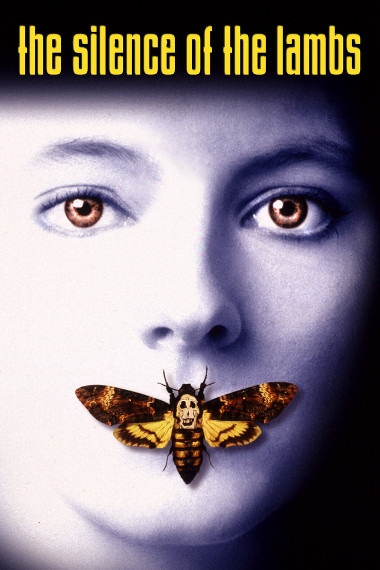
\includegraphics[width=0.19\textwidth]{affiches/silence.jpeg}
\end{tabular} 
\end{tabular}


\subsection{Films de Guerre}
\begin{tabular}{c c}
\begin{minipage}{12cm}
\RT{apocalypse_now}{\textcolor{blue}{Apocalypse Now}}  (Coppola) \beau \\
\RT{full_metal_jacket}{\textcolor{blue}{Full Metal Jacket}}  (\StanleyKubrick) \\
\RT{deer_hunter}{Voyage au Bout de l'Enfer}  (avec de Niro, \ChristopherWalken) \\
\RT{inglourious_basterds}{Inglorious Basterds} (et autres de Tarentino) \beau \\
\end{minipage}
\begin{tabular}{c}

\includegraphics[width=0.19\textwidth]{affiches/FMJ.jpg}
\end{tabular} 
\end{tabular}



\subsection{Westerns}
\subsubsection{Sérieux}
\RT{dances_with_wolves}{Danse avec les Loups} 
(de et avec Kevin Costner, Oscar meilleur film 1991) \beau \\
\RT{there_will_be_blood}{There Will Be Blood}  (2007, P.T. Anderson, avec Daniel Day Lewis)  --> à voir \beau \\

\subsubsection{Spaghettis (parodique)}
\textcolor{blue}{
La Trilogie du Dollar (Sergio Leone, avec Clint Eastwood): \beau
\begin{itemize}
\item \RT{fistful_of_dollars}{Pour une poignée de dollars} (1964)
\item \RT{for_a_few_dollars_more}{Et pour quelques Dollars de plus} (1965)
\item \RT{good_the_bad_and_the_ugly}{Le Bon, la Brute et le Truand} (1966)
\end{itemize} }
\RT{high_plains_drifter}{L'Homme des Hautes Plaines}  (de et avec Clint Eastwood) \beau \\
\RT{1041911-unforgiven}{Impitoyable} 
 (de et avec Clint Eastwood, Oscar meilleur film 1992) \\

\subsubsection{Néowesterns}
\RT{three_burials_of_melquiades_estrada}{Trois Enterrements} 
(de et avec Tommy Lee Jones) \\
\RT{1074022-lone_star}{Lone Star}

\subsection{Aventure et divertissement familial}
\href{https://www.rottentomatoes.com/search/?search=indiana+jones&sitesearch=rt}{Indiana Jones 1, 2 et 3}
(Spielberg) \\
\href{https://www.rottentomatoes.com/search/?search=pirates+of+the+caribbean&sitesearch=rt}{Pirates des Caraïbes 1, 2 et 3} \\
Be Kind, Rewind (Michel Gondry) \\

\subsection{Animés}
La plupart des Miyasaki (Princesse Mononoke, Le Chateau dans le Ciel...)\\
Ghost in the Shell (le film, pas la série)\\

\subsection{Vieux classiques (noir et blanc)}
\begin{tabular}{c c}
\begin{minipage}{12cm}
\RT{1010792-its_a_wonderful_life}{La Vie est Belle} (Capra, 1946) \\
\RT{1003707-casablanca}{Casablanca} (Michael Curtiz, 1942) \\
\RT{citizen_kane}{Citizen Kane}  (\OrsonWelles, 1941) \beau \\
\RT{lady_from_shanghai}{The Lady from Shanghai} (\OrsonWelles, 1948) \\
\RT{1000013-12_angry_men}{12 Hommes en Colère} (Sidney Lumet, 1957)\\
\RT{some_like_it_hot}{Certains l'aiment Chaud} (Billy Wilder, 1957) \\
\RT{rashomon}{Rashomon}  (Akira Kurosawa, 1951) \\
\RT{1018639-seven_samurai}{Les 7 Samourais}  (Akira Kurosawa, 1954) \\
Un Chien Andalou (Luis Bunuel)(à voir pour sa culture ciné) \\
\end{minipage}
\begin{tabular}{c}
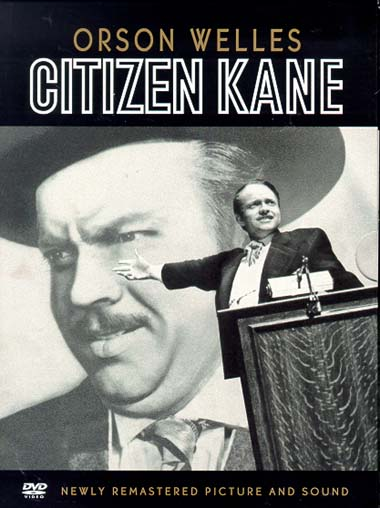
\includegraphics[width=0.19\textwidth]{affiches/citizenkane.jpg}
\end{tabular} 
\end{tabular}

\newpage
\section{Films français}
\subsection{Comédies}
\TRtele{le-nom-des-gens,17204080.php}{Le Nom des Gens}
(2010, avec Jacques Gamblin) \\
\TR{le-bruit-des-gla-ons,414024.php}{Le Bruit des Glaçons}
 (2010, Bertrand Blier, avec Jean Dujardin, Albert Dupontel)\\
\TRtele{intouchables,29464803.php}{Intouchables}
(2011, avec François Cluzet)  \\
\TR{the-artist,428139.php}{The Artist} 
(2011, Michel Hazanavicius, avec Jean Dujardin) \\
L'Arnacoeur (Romain Duris) \\
\TR{un-singe-en-hiver,42689.php}{Un Singe en Hiver} (1962, avec Jean-Paul Belmondo, Jean Gabin)\\  -> dialogues excellents (Audiard), musique très sympa \\
\TR{fais-moi-plaisir,382359.php}{Fais Moi Plaisir}(2009) \\
\TRtele{rire-et-chatiment,1701812.php}{Rire et Châtiment}
(2003, avec José Garcia) \\
\TR{le-diner-de-cons,43753.php}{Le Diner de Cons}
(1997, avec Jacques Villeret) \\
Le Concert (2009, Radu Mihaileanu) \\


\subsection{Comédies dramatiques}
\TR{le-fabuleux-destin-d-am-lie-poulain,54074.php}{Amélie Poulain}  (2000, JP Jeunet) \\
\TR{l-auberge-espagnole,60443.php}{L'Auberge Espagnole} (2002, Cédric Klapisch) \\
\TR{mon-oncle-d-amerique,8936.php}{Mon Oncle d'Amérique} (1980, Alain Resnais, avec Depardieu) \\
Tournée (Mathieu Amalric) \beau \\
\TR{mammuth,405676.php}{Mammuth} (2010, Délépine et Kervern, avec Gérard Depardieu) \\
\TR{louise-michel,359692.php}{Louise-Michel} (2007, Délépine et Kervern) \\
% le grand soir

\subsection{Drames}
\begin{tabular}{c c}
\begin{minipage}{12cm}
\TR{pierrot-le-fou-version-restauree,4609.php}{Pierrot le Fou} (1965, Godard) \beau \beau\\
\TR{le-mepris,4799.php}{Le Mépris} 
(1963, Godard) \beau \beau \\
\TR{des-hommes-et-des-dieux,196039.php}{Des Hommes et des Dieux}
(2010, avec Michael Lonsdale) \beau  \\
\TR{la-journee-de-la-jupe,374390.php}{La Journée de la Jupe}
(2008) \\
\TR{tous-les-matins-du-monde,8360.php}{Tous les Matins du Monde}
(1991, avec Gérard Depardieu) \\
\TR{le-chat,15925.php}{Le Chat} (1971) (avec Jean Gabin, Simone Signoret) \\
\TR{les-grandes-personnes,347066.php}{Les Grandes Personnes} (2008, avec JP Darroussin) \\
\TRtele{polisse,27602990.php}{Polisse} 
(2011) \\
\end{minipage}
\begin{tabular}{c}
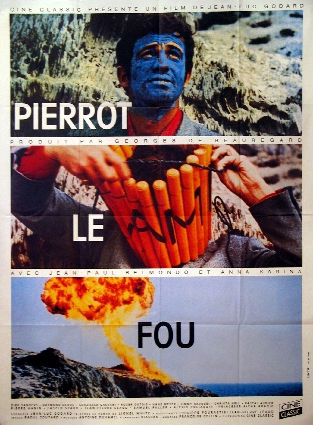
\includegraphics[width=0.20\textwidth]{affiches/pierrot.jpg}
\end{tabular} 
\end{tabular}


\subsection{Policier}
\TR{le-samoura,16660.php}{Le Samouraï}
(1967) (et autres de Jean-Pierre Melville) \beau \beau \\
\TRtele{garde-a-vue,27596.php}{Garde à Vue}
(1981, Claude Miller, avec Michel Serrault, Gérard Depardieu) \\

\subsection{Films à sketches}
Astérix et Obélix Mission Cléopâtre \\
2h moins le quart avant Jésus-Christ (Coluche)\\

\subsection{Autres}
\TR{le-crabe-tambour,47984.php}{Le Crabe-Tambour}
(1977, Pierre Schoenderffer) \\
\TRtele{les-derniers-jours-du-monde,13356921.php}{Les Derniers Jours du Monde}
(2009, SF, avec Mathieu Amalric) \\

\subsection{Vieux classiques (noir et blanc)}
\TR{les-tontons-flingueurs,14855.php}{Les Tontons Flingueurs}
(1963, Lautner, Audiard, avec Lino Ventura) \\
\TR{le-soupirant-en-version-restauree,14179.php}{Le Soupirant} (1962, Pierre Etaix) \beau  \\
\TR{lola,9759.php}{Lola}
(1961) (et autres de Jacques Demy) \beau  \\ \\ \\
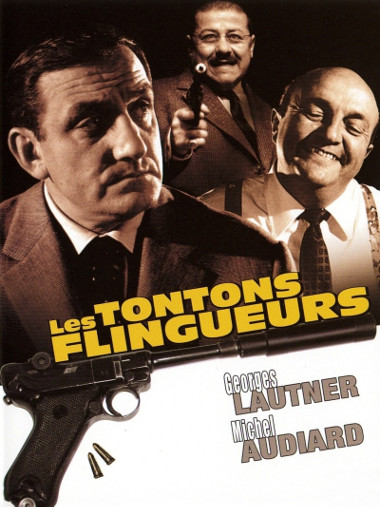
\includegraphics[width=0.38\textwidth]{affiches/tontons.jpg}


% !TeX root = main.tex

\newpage
\section{Réalisateurs (et mes films préférés)}
% ATTENTION: des tableaux trop longs pour une seule page peuvent causer des bugs:
% apparition de pages complètement vides
\begin{tabular}{c c}
\begin{tabular}{c}  % LIGNE 1
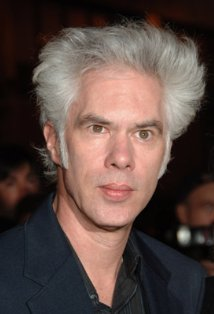
\includegraphics[width=0.15\textwidth]{acteurs/JJ.jpg}
\end{tabular} 
\begin{minipage}{4,5cm}
\JimJarmusch
\begin{itemize}
\item Ghost Dog
\item Broken Flowers
\item Mystery Train
\item Dead Man
\end{itemize}
\end{minipage} & 
\begin{tabular}{c}

\includegraphics[width=0.15\textwidth]{acteurs/TG.jpg}
\end{tabular} 
\begin{minipage}{10cm}
\acteur{terry_gilliam}{Terry Gilliam}
\begin{itemize}
\item Brazil
\item 12 Monkeys
\item Sacré Graal
\end{itemize}
\end{minipage} \\ \\
\begin{tabular}{c}  % LIGNE 2
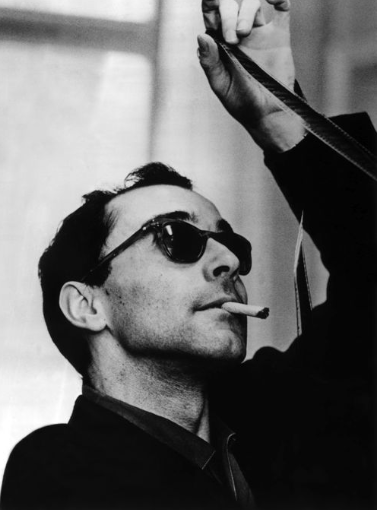
\includegraphics[width=0.15\textwidth]{acteurs/JLG.png}
\end{tabular} 
\begin{minipage}{4,5cm}
\acteur{jeanluc_godard}{Jean-Luc Godard} 
\begin{itemize}
\item Pierrot le Fou
\item Le Mépris
\item A Bout de Souffle
\end{itemize}
\end{minipage} &
\begin{tabular}{c}
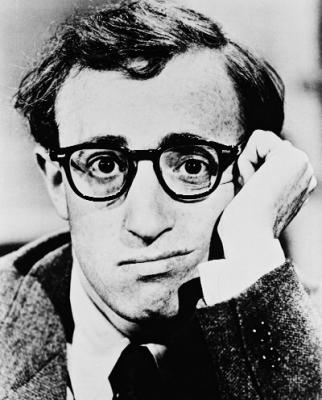
\includegraphics[width=0.15\textwidth]{acteurs/WA.jpg}
\end{tabular} 
\begin{minipage}{10cm}
\acteur{woody_allen}{Woody Allen}
\begin{itemize}
\item Midnight in Paris
\item Scoop
\item Whatever Works
\item Escrocs mais pas trop
\end{itemize}
\end{minipage} \\ \\
\begin{tabular}{c}  % LIGNE 3
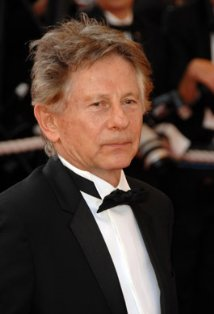
\includegraphics[width=0.15\textwidth]{acteurs/RP.jpg}
\end{tabular} 
\begin{minipage}{4,5cm}
\RomanPolanski
\begin{itemize}
\item Rosemary's Baby
\item Le Locataire
\item Le Bal des Vampires
\item Le Pianiste
\item Chinatown
\end{itemize}
\end{minipage} & 
\begin{tabular}{c}
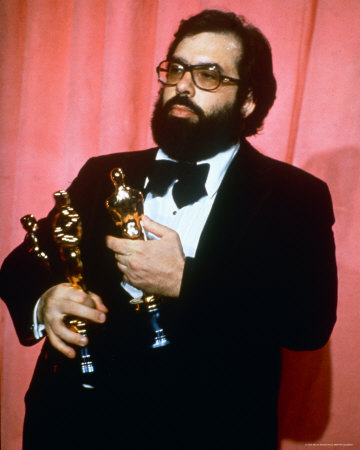
\includegraphics[width=0.15\textwidth]{acteurs/FFC.jpg}
\end{tabular} 
\begin{minipage}{10cm}
\acteur{francis_ford_coppola}{Francis Ford Coppola}
\begin{itemize}
\item Apocalypse Now
\item Tetro
\item Le Parrain
\item Conversation Secrète
\end{itemize}
\end{minipage} \\ \\
\begin{tabular}{c}  % LIGNE 4
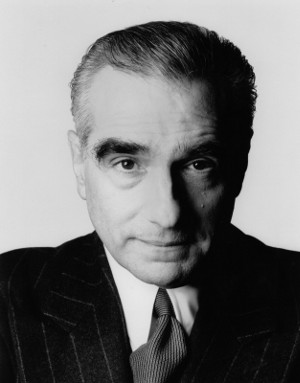
\includegraphics[width=0.15\textwidth]{acteurs/MS.jpeg}
\end{tabular} 
\begin{minipage}{4,5cm}
\MartinScorsese
\begin{itemize}
\item Taxi Driver
\item Les Affranchis
\item Les Infiltrés
\end{itemize}
\end{minipage} & 
\begin{tabular}{c}
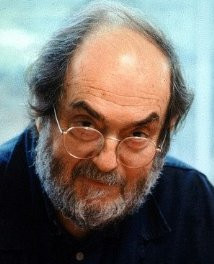
\includegraphics[width=0.15\textwidth]{acteurs/kubrick.jpeg}
\end{tabular} 
\begin{minipage}{10cm}
\StanleyKubrick
\begin{itemize}
\item Full Metal Jacket
\item Docteur Folamour
\item Orange Mécanique
\item Shining
\item 2001
\end{itemize}
\end{minipage} \\ \\
\begin{tabular}{c}  % LIGNE 5
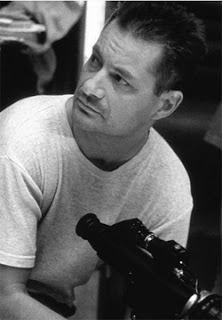
\includegraphics[width=0.15\textwidth]{acteurs/JPJ.jpg}
\end{tabular} 
\begin{minipage}{4,5cm}
\acteur{jeanpierre_jeunet}{Jean-Pierre Jeunet}
\begin{itemize}
\item Amélie Poulain
\item Délicatessen
\item Alien IV
\item La Cité des Enfants Perdus
\end{itemize}
\end{minipage} & 
\begin{tabular}{c}
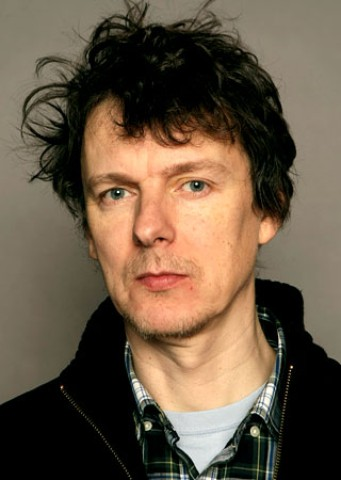
\includegraphics[width=0.15\textwidth]{acteurs/MG.jpg}
\end{tabular} 
\begin{minipage}{10cm}
\acteur{michel_gondry}{Michel Gondry} 
\begin{itemize}
\item Eternal Sunshine
\item Be Kind, Rewind
\item La Science des Rêves
\end{itemize}
\end{minipage} \\ \\
\begin{tabular}{c}  % LIGNE 6
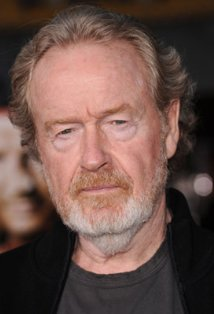
\includegraphics[width=0.15\textwidth]{acteurs/RS.jpg}
\end{tabular} 
\begin{minipage}{4,5cm}
\acteur{ridley_scott}{Ridley Scott}
\begin{itemize}
\item Blade Runner
\item Alien
\item Thelma \& Louise
\end{itemize}
\end{minipage} & 
\begin{tabular}{c}
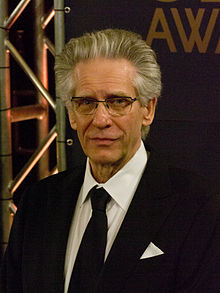
\includegraphics[width=0.15\textwidth]{acteurs/DC.jpeg}
\end{tabular} 
\begin{minipage}{10cm}
\DavidCronemberg
\begin{itemize}
\item eXistenZ
\item Cosmopolis
\item A History of Violence
\item Videodrome
\end{itemize}
\end{minipage}
\end{tabular}

\newpage % REALISATEURS PAGE 2
\begin{tabular}{c c}
\begin{tabular}{c}
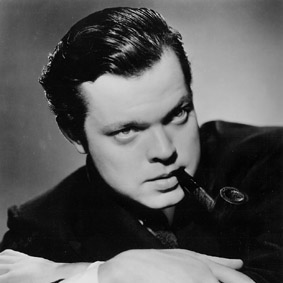
\includegraphics[width=0.15\textwidth]{acteurs/OW.jpg}
\end{tabular} 
\begin{minipage}{4,5cm}
\acteur{orson_welles}{Orson Welles}
\begin{itemize}
\item Citizen Kane
\item Le Procès
\item La Dame de Shanghai
%\item Le Procès
\end{itemize}
\end{minipage} & 
\begin{tabular}{c}
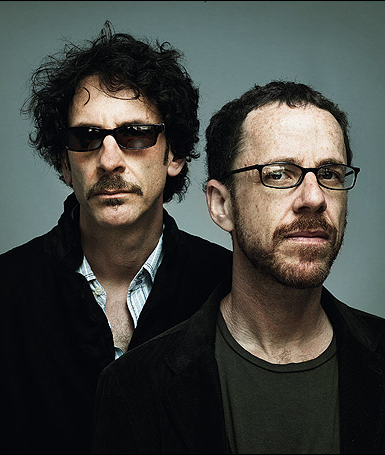
\includegraphics[width=0.15\textwidth]{acteurs/FC.png}
\end{tabular} 
\begin{minipage}{10cm}
\acteur{joel_coen}{Frères Coen}
\begin{itemize}
\item The Big Lebowski
\item The Barber
\item No Country For Old Men
\item Barton Fink
\end{itemize}
\end{minipage} \\ \\
\end{tabular} \\ \\ \\
% potentiels: takeshi kitano
Et aussi:\\
Darren Arronovski (Requiem for a Dream, Black Swan, The Wrestler...)\\
David Lynch (Elephant Man, Mulholland Drive, Blue Velvet...)\\
Almodovar (Volver, Femmes au bord de la crise de nerfs...)\\
Peter Weier (Witness, Dead Poets Society, Etat Second...)\\
Kenneth Brannagh (Le Limier, Beaucoup de Bruit pour rien, Dead Again...)\\
Takeshi Kitano (Aniki mon Frère, Hana-Bi)\\ % sonatine, dolls
Zhang Yimou (Hero, La Cité Interdite...)\\
Tarentino (Inglorious Basterds, Pulp Fiction, Kill Bill, Reservoir Dogs...)\\
Robert Rodriguez (Machete, Sin City, From Dusk till Dawn)\\
Hayao Miyasaki (Princesse Mononoke, Le Chateau Ambulant, Nausicaa, Le Chateau dans le Ciel, Le Voyage de Chihiro...)\\ \\ \\

\href{http://www.youtube.com/watch?v=CAKS3rdYTpI}{Voir ici un commentaire de Terry Gilliam sur Spielberg} \\


% !TeX root = main.tex

\newpage
\section{Acteurs/actrices préférés}
\subsection{Acteurs}
\begin{tabular}{*{5}{c}}
% LIGNE 1
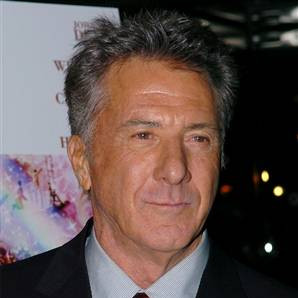
\includegraphics[width=0.15\textwidth]{acteurs/DH.jpg} 
& 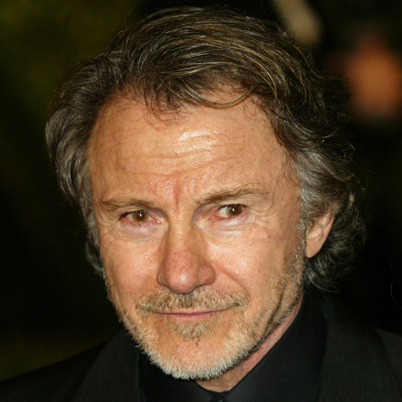
\includegraphics[width=0.15\textwidth]{acteurs/HK.jpg} 
& 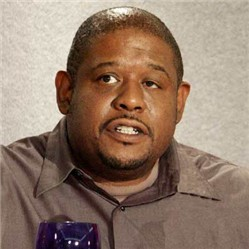
\includegraphics[width=0.15\textwidth]{acteurs/FW.jpg} 
& 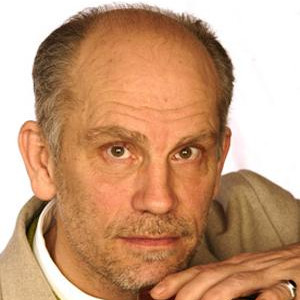
\includegraphics[width=0.15\textwidth]{acteurs/JM.jpg} 
& 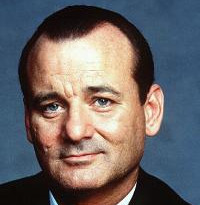
\includegraphics[width=0.15\textwidth]{acteurs/BM.jpg} \\
\acteur{dustin_hoffman}{Dustin Hoffman} 
& \acteur{harvey_keytel}{Harvey Keitel}
& \acteur{forest_whitaker}{Forest Whitaker}
& \acteur{john_malkovich}{John Malkovich} 
& \acteur{bill_murray}{Bill Murray} \\ \\

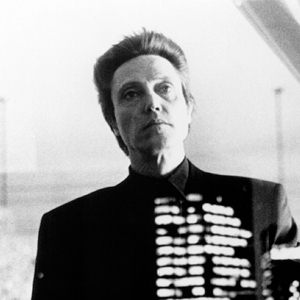
\includegraphics[width=0.15\textwidth]{acteurs/CW.jpg} 
& 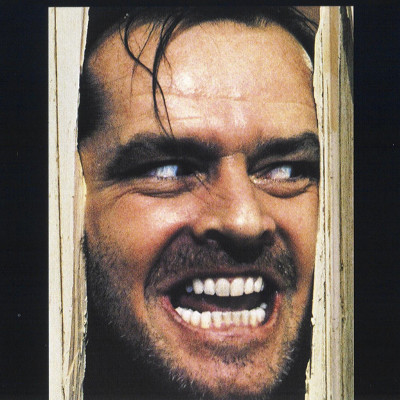
\includegraphics[width=0.15\textwidth]{acteurs/JN.jpg} 
& 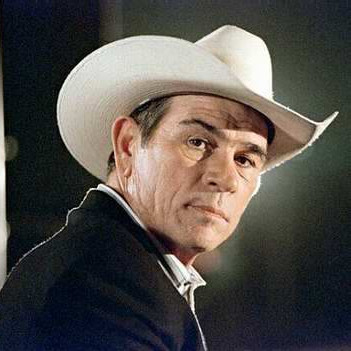
\includegraphics[width=0.15\textwidth]{acteurs/TLJ.jpg} 
& 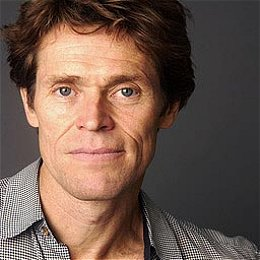
\includegraphics[width=0.15\textwidth]{acteurs/WD.jpg} 
& 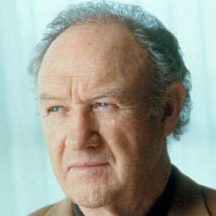
\includegraphics[width=0.15\textwidth]{acteurs/GH.jpg} \\
\acteur{christopher_walken}{Christopher Walken} 
& \JackNicholson
& \acteur{tommy_lee_jones}{Tommy Lee Jones}
& \acteur{willem_dafoe}{Willem Dafoe} 
& \acteur{gene_hackman}{Gene Hackman} \\ \\

% LIGNE 2 (SECONDS ROLES)
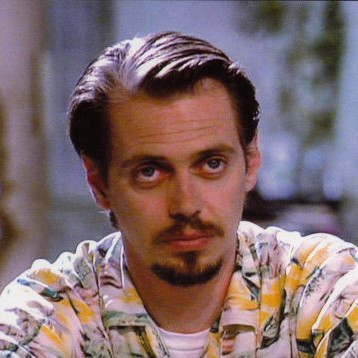
\includegraphics[width=0.15\textwidth]{acteurs/SB.jpg} 
& 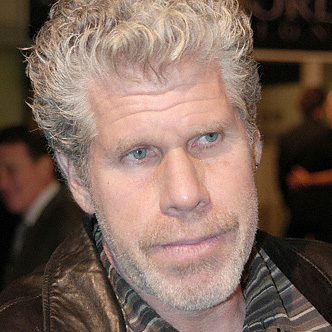
\includegraphics[width=0.15\textwidth]{acteurs/RP2.jpg} 
& 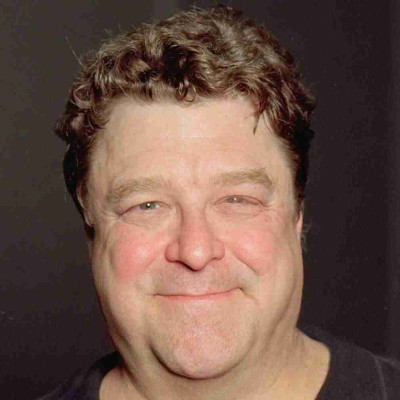
\includegraphics[width=0.15\textwidth]{acteurs/JG.jpg} 
& 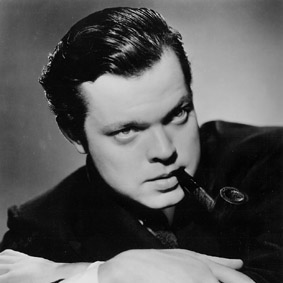
\includegraphics[width=0.15\textwidth]{acteurs/OW.jpg} 
& 
\includegraphics[width=0.15\textwidth]{acteurs/void.jpg} \\
 \acteur{steve_buscemi}{Steve Buscemi} 
& \acteur{ron_perlman}{Ron Perlman} 
& \acteur{john_goodman}{John Goodman}
& \acteur{orson_welles}{Orson Welles}
& \href{LIEN}{}\\
\end{tabular}\\ \\ \\


Et aussi:\\
Sean Penn (21 Grammes, Mystic River...)\\
Christoph Waltz (Inglorious Basterds, Django) \\
Adrien Brody (Le Pianiste, The Darjeeling Limited...)\\
Al Pacino (Insomnia, Heat, Le Parrain...)\\
Clint Eastwood (pour ses westerns spaghettis et Dirty Harry)\\
Klaus Kinski (Aguirre, Et pour quelques dollars de plus...)\\
Carmen Maura (Volver et autres de Pedro Almodovar)\\
Javier Bardem (Mar Adentro...)\\
Joaquin Phoenix (Two Lovers)\\
Benicio del Toro (21 Grammes...)\\
Mads Mikkelsen (Casino Royale)\\
Jude Law (Gattaca...)\\
Ralph Fiennes (The Constant Gardener, Le Patient Anglais...)\\
Emma Thomson\\
Robin Williams (Insomnia, Dead Poets Society...)\\
Anthony Hopkins (Le Silence des Agneaux, Elephant Man...)\\
John Cazale (Le Parrain, The Deer Hunter, Conversation Secrète)\\
Kevin Spacey\\
Michael Lonsdale (Le Nom de la Rose, Des Hommes et des Dieux)\\

Fabrice Luchini\\
Jacques Gamblin (Le Nom des Gens)\\
Mathieu Amalric (Les Derniers Jours du Monde, Tournée...)\\
François Cluzet\\
Grégory Gadebois (Rapace)\\
Julie Delpy (Two Days in Paris...)\\
Isabelle Carre\\
Audrey Tautou (Amélie Poulain, Hors de Prix, Ensemble c'est Tout...)\\

\subsection{Actrices}
\begin{tabular}{*{5}{c}}
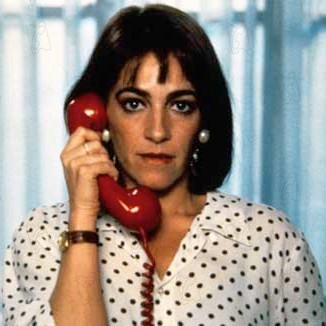
\includegraphics[width=0.15\textwidth]{acteurs/CM.jpg} 
& 
\includegraphics[width=0.15\textwidth]{acteurs/void.jpg} 
& 
\includegraphics[width=0.15\textwidth]{acteurs/void.jpg} 
& 
\includegraphics[width=0.15\textwidth]{acteurs/void.jpg} 
& 
\includegraphics[width=0.15\textwidth]{acteurs/void.jpg} \\
 \acteur{carmen_maura}{Carmen Maura} 
& \href{LIEN}{} 
& \href{LIEN}{}
& \href{LIEN}{}
& \href{LIEN}{}\\
\end{tabular}

% TODO: ajouter:
% michael londsale
% ana karina


\newpage
\section{Autres}
\subsection{Séries}
\begin{itemize}
\item Dexter
\item Docteur House (surtout la saison 4)
\item How I met your Mother
\item The Big Bang Theory
\item Scrubs
\end{itemize}

\subsection{Humoristes}
\begin{itemize}
\item Stéphane Guillon (le spectacle "En avant la Musique")
\item Fabrice Eboué
\end{itemize}

\subsection{Documentaires}
\begin{itemize}
\item Zétwal
\end{itemize}

\subsection{Court-métrages}
\href{http://www.dailymotion.com/video/xchpac_garde-fou_shortfilms}{Garde-fou (très original)}

\subsection{Sites internet}
\href{https://www.rottentomatoes.com/}{RottenTomatoes}: site US de critiques (compile les critiques de plusieurs sources)\\
\href{http://www.metacritic.com/}{Metacritic}: idem que RottenTomatoes. Valable aussi pour les séries télé et la musique\\
\href{http://www.telerama.fr/}{Télérama}: journal français de critiques\\
\href{http://iwdrm.tumblr.com/}{IWDRM}: des scènes cultes en .gif\\

\subsection{Films avec bonne BO}
\begin{itemize}
\item Le Lauréat: Simon \& Garfunkel
\item Ghost Dog: RZA \& The Wu Tang Clan
\item Drive: Kavinsky
\item Les films de Tarentino (Pulp Fiction...)
\item The Darjeeling Limited: musiques indiennes
\end{itemize}

\subsection{Jeux vidéo}
\href{http://www.jeuxvideo.com/jeux/playstation-3-ps3/00037095-classics-hd-ico-shadow-of-the-colossus.htm}{Shadow of the Colossus}: jeu très poétique. Voir aussi Ico, de la même équipe.\\
\href{http://www.jeuxvideo.com/jeux/playstation-3-ps3/00020227-portal.htm}{Portal}: jeu de réflexion\\
Metal Gear Solid 1, 2, 3 et 4: les classiques des jeux d'infiltration\\
Dead Space 1 et 2: survival-horror dans un univers inspiré d'Alien. Une vraie direction artistique pour les graphismes.\\
Demon's Souls et Dark Souls: RPG bien pensés sans baratin et pertes de temps inutiles.\\
Antichamber: jeu de réflexion assez philosophique.\\
Et aussi: Limbo, Flower...\\

\subsection{Littérature}
Cyrano de Bergerac, la pièce d'Edmond Rostand\\
Antigone, la pièce de Jean Anouilh\\
Balzac et la petite tailleuse chinoise (roman, Dai Sijie)\\
La grammaire est une chanson douce (roman, Erik Orsenna)\\

\subsection{BD}
Deathnote (manga): histoire très complexe et pourtant très cohérente. Et seulement 12 tomes, donc pas besoin de se ruiner.\\
Broussailles (les albums "Les baleines publiques" et "La nuit du chat"). Assez poétique.\\

%\newpage
%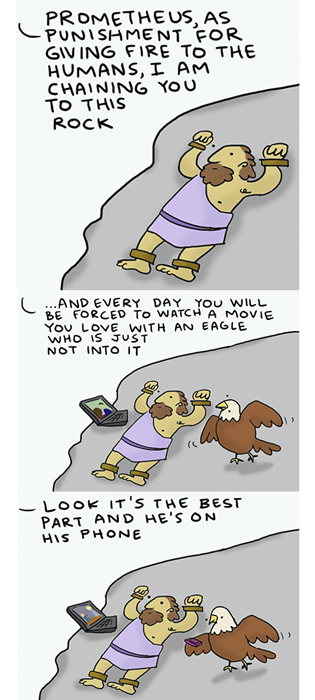
\includegraphics[width=0.70\textwidth]{humour/prometheus.png}

%\newpage
%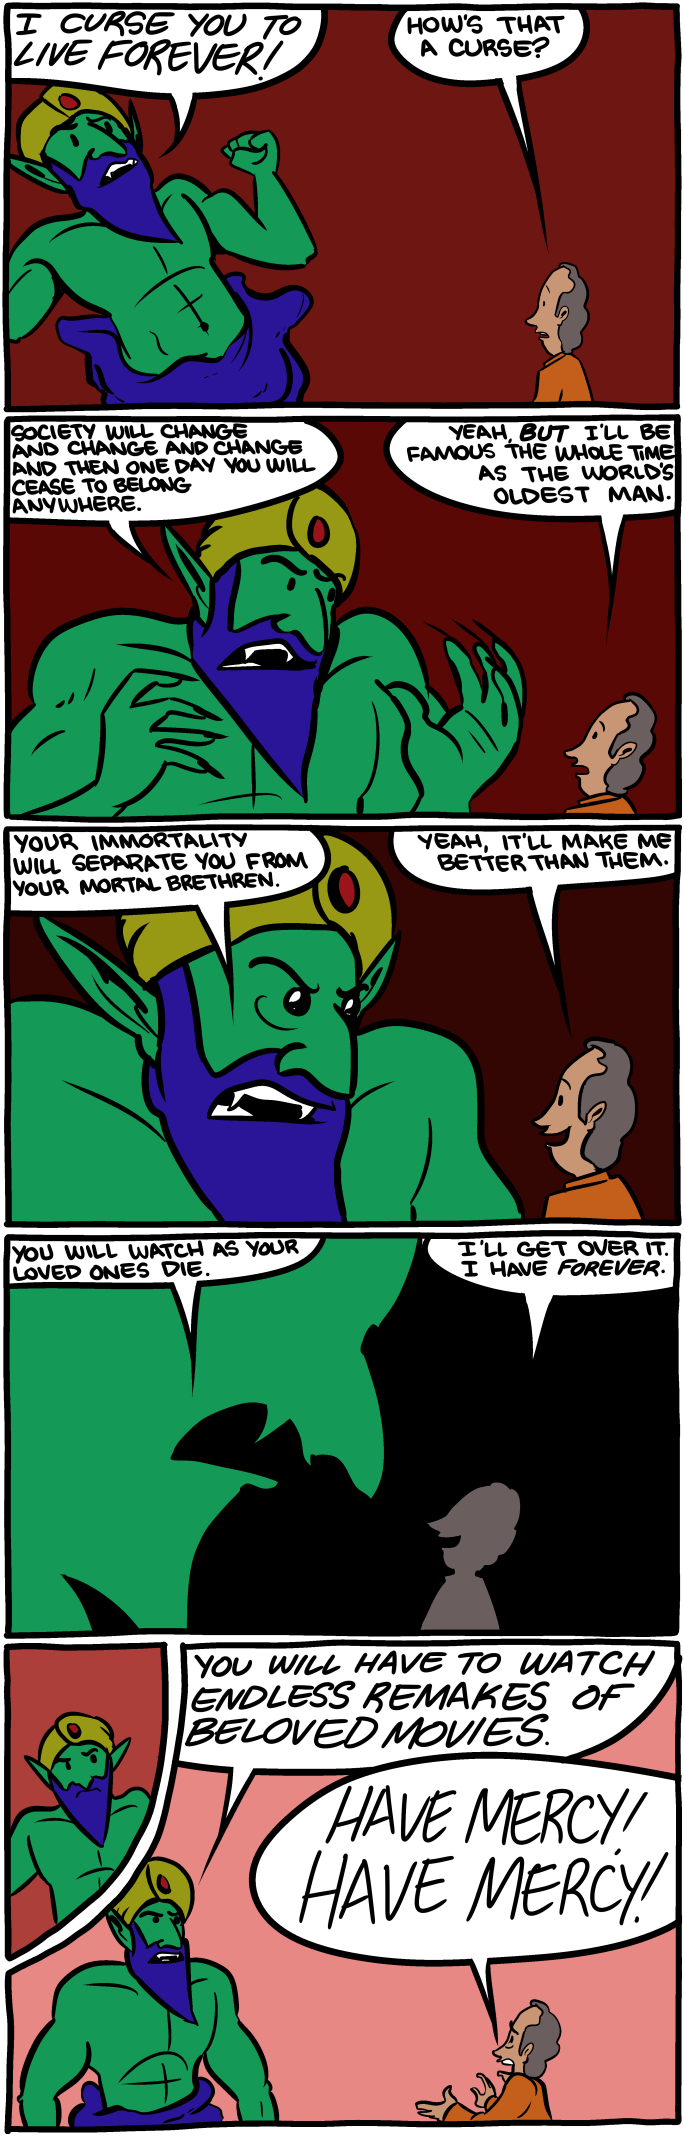
\includegraphics[width=0.50\textwidth]{humour/smbc-remakes.png}

%\newpage
%\section*{Conclusion}
%\addcontentsline{toc}{section}{Conclusion}


\end{document}
